The FEM panel will present users with a selection of FEM
applications. Currently, there is two application
available, OpenSees and FEAPpv. More FE platforms will be added 
 in future versions to allow users to provide their own
simulation application.  

\begin{figure}[!htbp]
  \centering {
    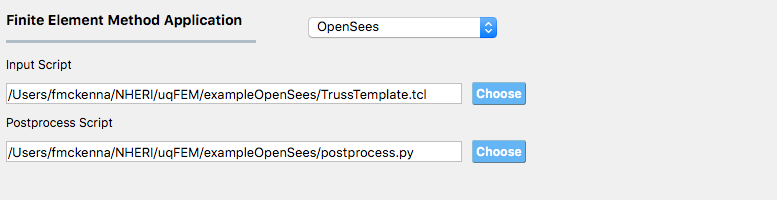
\includegraphics[width=0.8\textwidth]
    {examples/fig_quofem/fem.png} }
  \caption{Options for FEM file specification with OpenSees}
  \label{fig:fem}
\end{figure}

\begin{figure}[!htbp]
  \centering {
    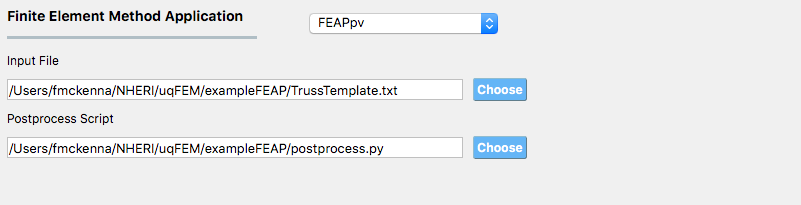
\includegraphics[width=0.8\textwidth]
    {examples/fig_quofem/fem2.png} }
  \caption{Options for FEM file specification with FEAPpv}
  \label{fig:fem2}
\end{figure}

For the OpenSees and FEAPpv applications, the user is required to specify the FEM input file, as shown in \Cref{fig:fem} and \Cref{fig:fem2}, respectively. A user-provided post-processing script for each FEM application needs to be selected appropriately. 